\documentclass[numbers=noenddot,14pt,a4paper]{scrartcl}
\usepackage[greek,ngerman]{babel}
\usepackage[T1]{fontenc}
\usepackage[utf8]{inputenc}
\usepackage{fullpage}
\usepackage{libertine}
\usepackage{ziffer}
\usepackage{graphicx}
\usepackage{units}
\usepackage[infoshow]{tabularx}
\usepackage{amsmath}
\usepackage{amssymb}
\usepackage{wrapfig}
\usepackage{esint}
\usepackage{float}
\usepackage{wrapfig}
\usepackage[font=small]{caption}
\usepackage{subcaption}
\usepackage{lscape}
\usepackage{hyperref}

\renewcommand{\thefigure}{Abb. \arabic{figure}}

\captionsetup[wrapfigure]{name=}
\captionsetup[figure]{name=}
\newcommand{\degree}{^\circ}
\newcommand{\diff}{\textnormal{d}}
\newcommand{\tenpo}[1]{\cdot 10^{#1}}
\newcommand{\greek}[1]{\greektext#1\latintext}
\newcommand{\ix}[1]{_\text{#1}}
\newcommand{\imag}{\mathbf{i}}
\newcommand{\tilt}[1]{\textit{#1}}
\newcommand{\grad}[1]{\textit{grad}\left(#1\right)}
\newcommand{\divergenz}[1]{\textit{div}\left(#1\right)}
\newcommand{\euler}{\mathnormal{e}}
\newcommand{\fett}[1]{\textbf{#1}}

\title{Protokoll: Hall-Effekt in Halbleitern} %TODO Name des Versuchs eintragen
\author{Tom Kranz, \underline{Philipp Hacker}}
\date{\today}

\begin{document}
%\setcounter{page}{2}
%\setcounter{section}{1}
\maketitle
\begin{center}
Betreuer: Dr. Marvin von der Ehe\\ %TODO Name des Betreuers eintragen
Versuchsdatum: 18.11.2014\\ %TODO Datum des Versuchs eintragen
\begin{table}[h]
\centering
Note: %TODO Gute Note erhalten :)
\begin{tabularx}{1.5cm}{|X|}
\hline \\ \\
\hline
\end{tabularx}
\end{table}
\end{center}
\vspace*{\fill}
\tableofcontents
\vfill
\newpage
\section{Einleitung}
Dem sog. \tilt{Hall-Effekt} bedient man sich bei der Messung von magnetischen Feldstärken. Dabei werden Halbleiter eingesetzt, die in ihren attraktiven Eigenschaften sich dafür sehr gut eignen. In diesem Versuch sollen die Prinzipien dieser Vorgehensweise und die Unterschiede zwischen verschieden \tilt{dotierten} Materialien aufgezeigt werden. Im Fokus stehen außerdem die Untersuchungen von Beweglichkeit der Ladungsträger, der Konzentrationen dieser und deren Rückschlüsse auf interne Stromflussprozesse im Halbleiter.
\section{Durchführung}
\section{Physikalische Grundlagen}
\subsection{Halbleiter}
\begin{wrapfigure}[15]{ro}{0.5\textwidth}
	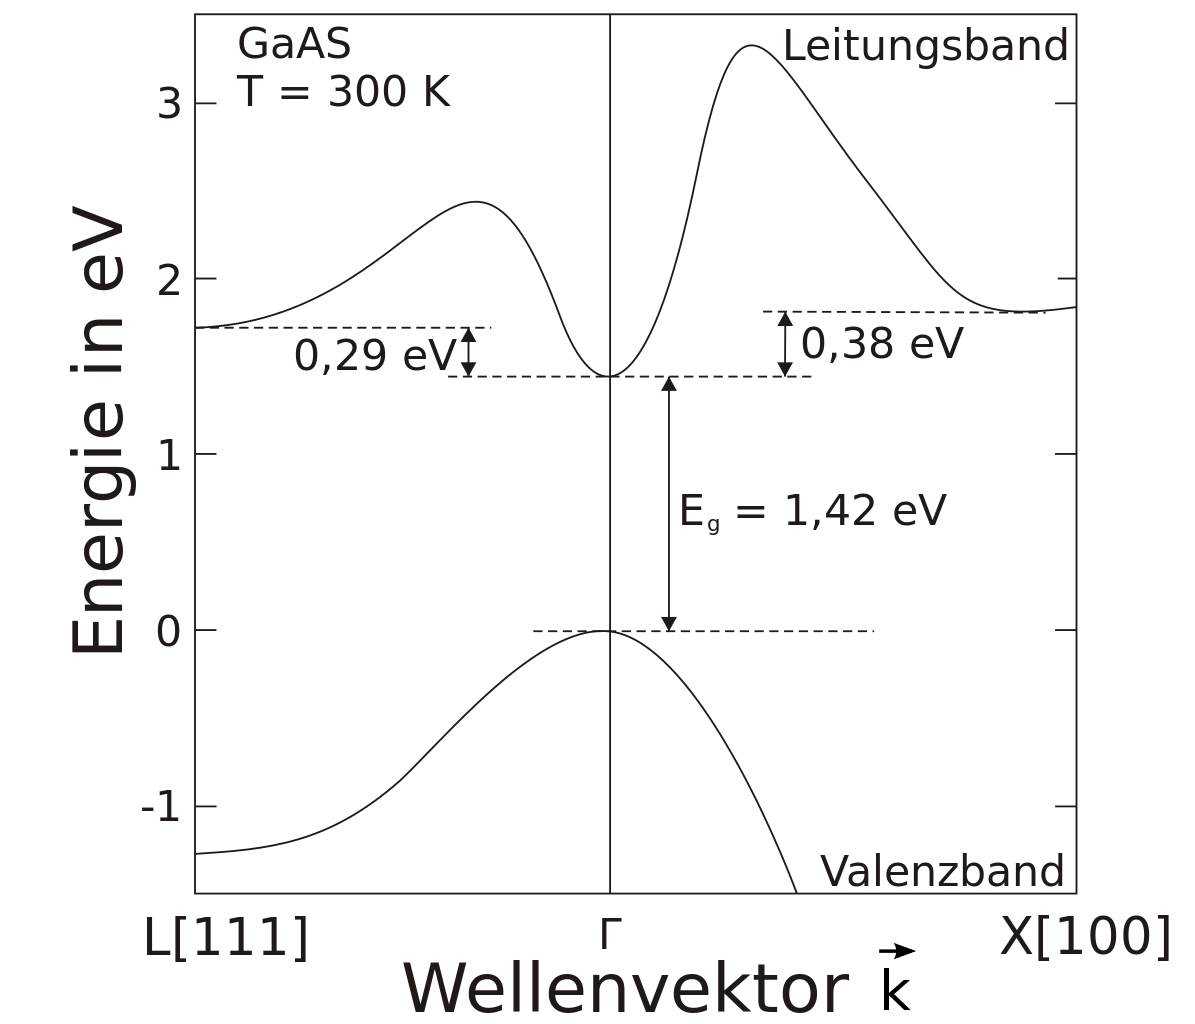
\includegraphics[width=0.5\textwidth]{Bandstruktur_GaAs.png}
	\caption{reduzierte Bandstruktur in Silizium mit eingezeichneten Richtungsachsen}
	 \label{img:band}
\end{wrapfigure}
Halbleiter sind Festkörper, welche sich durch eine kleine, nicht von Ladungsträgern besiedelten Energielücke $E\ix{G}$ zwischen dem letzten besetzen Energieband, dem \tilt{Valenzband}, und dem darauf folgendem, dem \tilt{Leitungsband} charakterisieren (\ref{img:band}). Nach \tilt{Wolfgang Pauli} (1925) kann das $N$-te Band maximal mit $2N$ verschiedenen Zuständen der Ladungsträger, den Elektronen besetzt werden. Diese werden in, an die Atome im Gitter des Halbleiter-Kristalls gebundene Rumpfelektronen und quasifreie, bewegliche Elektronen unterschieden.\\
In Halbleiter können damit bereits durch thermische Anregung oder kleine äußere Felder Elektronen in das Leitungsband übergehen und damit einen elektrischen Strom fließen lassen. Aus dem Übergang geht auch ein sog. \tilt{Defektelektron} hervor, was einen unbesetzten Zustand oder ein Loch im Band, aus welchen das Elektronen abwandert, ausdrückt und damit die Gleichheit von Loch- und Ladungsträgerkonzentration fordert. Diese wird als \tilt{intrinsische Ladungsträgerdichte} bezeichnet. Es sei angemerkt, dass die Bewegung der Elektronen, quantenmechanisch betrachtet, durch eine Welle mit Richtungsvektor $\vec{k}$ und der Winkelgeschwindigkeit $\omega$ ausgedrückt werden kann.\\
Betrachtet man die Defektelektronen als pos. Ladungen, so tragen sie unter einen äußeren elektrischen Feld $\vec{E}$ zu der Dichte des dabei fließenden Stromes $\vec{j}$ aus Gl. (\ref{eq:strom}) bei. Hierbei haben die Quasi"~/Teilchen einmal die Geschwindigkeit $\vec{v}\ix{n/p}$. Diese Eigenschaft nennt man \tilt{Eigentleitung} $\sigma\ix{i}$. Allgemein sind jedoch die Beweglichkeiten $\mu$ und Konzentrationen $p$ bzw. $n$ von Löchern und freien Elektronen nicht gleich (Verunreinigungen).
\begin{align}
	\vec{j}=q\ix{e}n\vec{v}\ix{n}+q\ix{p}p\vec{v}\ix{p}=e\left(n\mu\ix{n}+p\mu\ix{p}\right)\vec{E}=\sigma\vec{E} \label{eq:strom}
\end{align}
($\sigma$ - Leitfägikeit; $e$ - Elementarladung; $q\ix{i}$ - Ladung der Teilchen)
\subsection{Ladungsträgerdichten und Beweglichkeiten}
Da eine thermische  bzw. äußere Anregung nötig ist, um Elektronen ins Leitungsband zu bewegen, kann eine starke Temperaturabhängigkeit von $n$ und $p$ gefolgert werden. Die Besetzung der Energieniveaus muss der Fermi-Statistik $f\left(E,T\right)$ folgen. In der Regel ist jedoch die Aufweichung von $f\left(E,T\right)$ im Bereich $\sim2k\ix{B}T$ und damit sehr klein gegen $E\ix{G}$. Sie kann deswegen durch die Boltzmann-Statistik ersetzt werden, sofern $E-E\ix{F}>>2k\ix{B}T$ für die Fermi-Energie zwischen den Bändern gilt. Damit werden die Ladungsträgerdichten zu:
\begin{align}
	n=&\int_{E\ix{L}}^{\infty}D\ix{L}\left(E\right)\euler^{-\frac{E-E\ix{F}}{k\ix{B}T}}\diff E=\int_{E\ix{L}}^{\infty}\frac{\left(2m\ix{n}\right)^{3/2}}{2\pi^2\hbar^3}\sqrt{E-E\ix{L}}\euler^{-\frac{E-E\ix{F}}{k\ix{B}T}}\diff E \nonumber \\
	=&\frac{\left(2m\ix{n}k\ix{B}T\right)^{3/2}}{2\pi^2\hbar^3}\euler^{-\frac{E\ix{L}-E\ix{F}}{k\ix{B}T}}\int_{E\ix{L}}^{\infty}\sqrt{E-E\ix{L}}\euler^{-\frac{E}{k\ix{B}T}}\diff E \nonumber \\
	=&2\left(\frac{2\pi m\ix{n}k\ix{B}T}{h^2}\right)^{3/2}\euler^{-\frac{E-E\ix{F}}{k\ix{B}T}}=N^L\ix{eff}\euler^{-\frac{E-E\ix{F}}{k\ix{B}T}} \\
	\text{analog} \, \,\, p=&2\left(\frac{2\pi m\ix{p}k\ix{B}T}{h^2}\right)^{3/2}\euler^{-\frac{E\ix{V}-E\ix{F}}{k\ix{B}T}}=N^V\ix{eff}\euler^{-\frac{E\ix{V}-E\ix{F}}{k\ix{B}T}}
\end{align}
($D\ix{L/V}$ - Zustandsdichten in den Bändern; $m\ix{n/p}$ - effektive Massen; $E\ix{V}$,$E\ix{L}$ - Bandkanten)\\
Die Konzentrationen für quasifreie Ladungsträger folgen somit der Boltzmann-Statistik. Die Faktoren $N^{L/V}\ix{eff}$ sind die effektiven Zustandsdichten und gehen mit $T^{3/2}$. Man kann nun sich das jeweilige Band als ein einziges Energieniveau mit den betreffenden Zustandsdichten denken. Die Besetzungsdichte wird durch die Boltzmann-Verteilung geregelt. Beachtet werden muss jedoch, das ebenso $E\ix{F}$ als auch $E\ix{V/L}$ von außen verschoben werden können. Dem folgen die Integrale der Besetzungsdichten nach. Außerdem ist offensichtlich $E\ix{G}=E\ix{L}-E\ix{V}$.\\
Die besprochene intrinsische Ladungsträgerkonzentration wird damit zu
\begin{align}
	n\ix{i}=\sqrt{np}=\sqrt{4\left(\frac{k\ix{B}T}{2\pi\hbar^2}\right)^3\left(m\ix{n}m\ix{p}\right)^{3/2}\euler^{-\frac{E\ix{G}}{k\ix{B}T}}}=\sqrt{N^{V}\ix{eff}N^{L}\ix{eff}}\euler^{-\frac{E\ix{G}}{2k\ix{B}T}}
\end{align}
Die Beweglichkeiten $\mu\ix{n/p}$ sind Mittelwerte über die besetzten Zustände im Valenz- und Leitungsband. Löcher und Elektronen verhalten sich dabei qualitativ gleich. Es gilt wiederum die Boltzmann-Statistik für die folgenden Mittelwerte.
\begin{align}
	\mu=\frac{1}{m}\frac{\langle\tau(\vec{k}) v^2(\vec{k})\rangle}{\langle v^2(\vec{k})\rangle}
\end{align}
($\tau(\vec{k})$ - Relaxationszeit  des Elektrons am reziproken "`Ort"' $\vec{k}$)\\
Grob kann gefolgert werden, dass $\mu\sim\tau$. Jedoch ist $\tau$ proportional zur mittleren freien Weglänge der bewegten Ladungsträger.\\
Somit kann man $\frac{1}{\tau}\sim\langle v\rangle\Sigma$ für einen Streuquerschnitt der Teilchen $\Sigma$ als Stoßwahrscheinlichkeit auffassen. Außerdem ist, wegen der Boltzmann-Statistik der Bewegungen $\langle v\rangle\sim\sqrt{T}$. Nimmt man nun an, das die Streuung nur an Phononen oder ionisierten Störstellen stattfindet kann, so folgen 2 grundlegende Überlegungen:
\begin{itemize}
	\item{Streuquerschnitt eines Phonons mit ($\vec{q},\omega(\vec{q}))$ sei}
\end{itemize}
\section{Auswertung}
\section{Quellen}
\begin{itemize}
	\item{\url{http://de.wikipedia.org/wiki/Bandstruktur}\\ Abschn.: Bandstrukturen realer Festkörper}
\end{itemize}\end{document}